\begin{frame}
    \frametitle{485-x Makes 100 Units a Threshold}
    \begin{itemize}[itemsep=0.5em]
        \item New York City's main tax incentive for new rental housing, replacing 421-a in 2024
        \item Rental sites with 100 or more units face stricter affordability rules and a construction wage floor
        \item Sites can avoid the threshold by building fewer units or by dividing a project into smaller parts
    \end{itemize}
\end{frame}

\begin{frame}
    \frametitle{Developers Are Proposing 99-Unit Buildings}
    \begin{columns}[c,onlytextwidth]
        \begin{column}{0.52\textwidth}
            \centering
            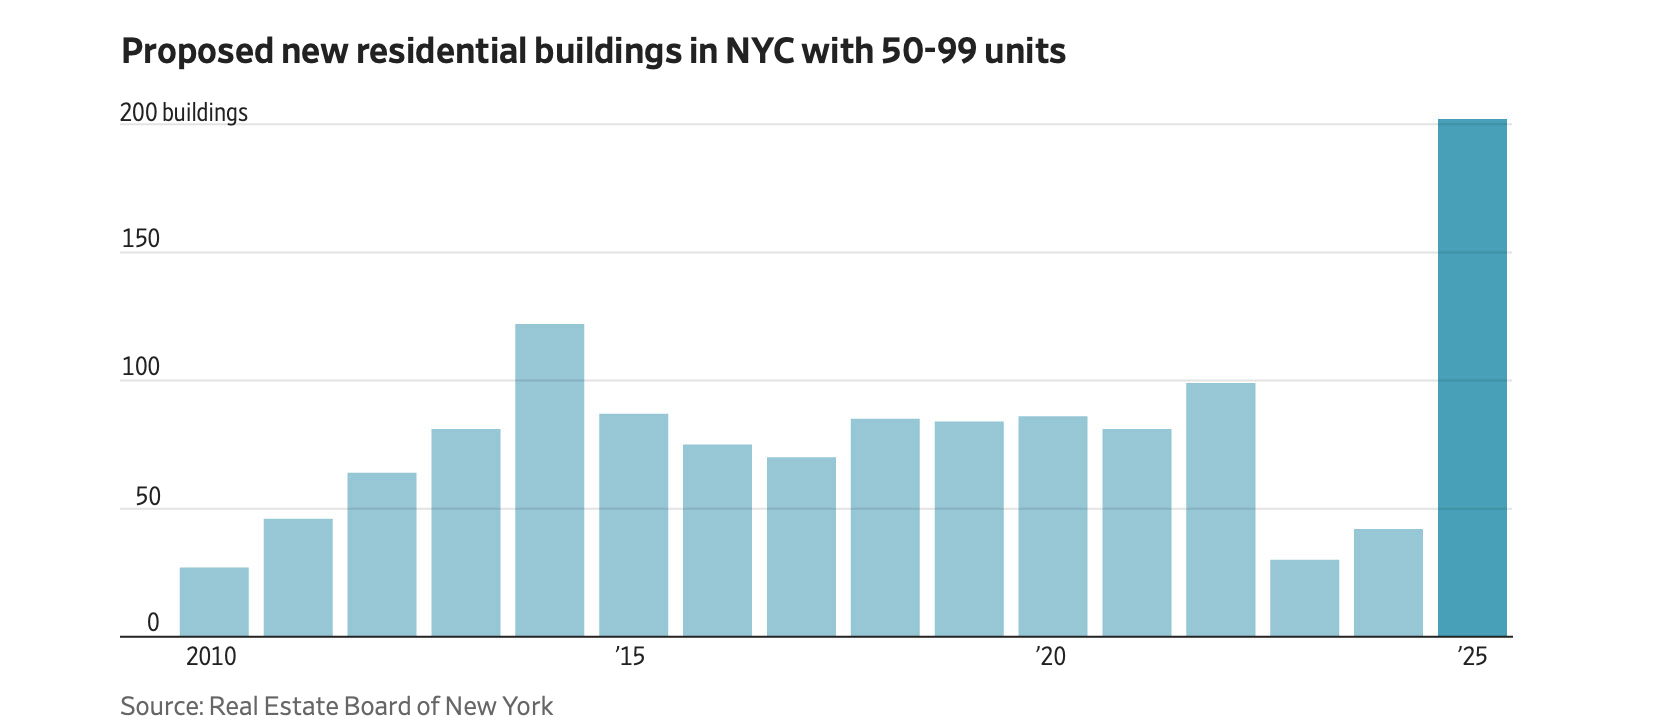
\includegraphics[width=\linewidth]{images/wsj_50_99_unit_buildings.png}
            \par\vspace{0.8em}
            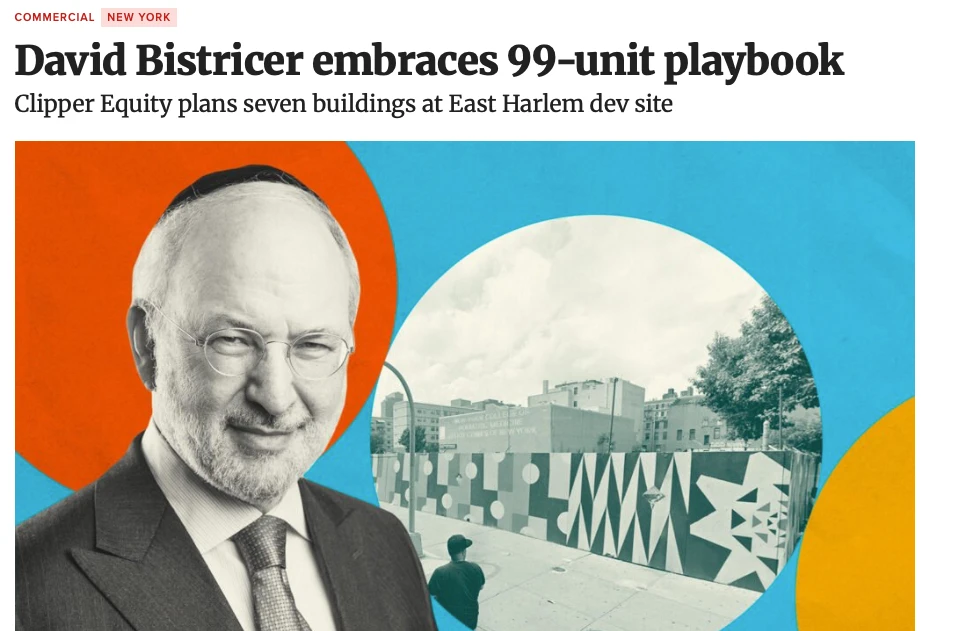
\includegraphics[width=\linewidth,height=0.4\textheight,keepaspectratio]{images/real_deal_bistricer_99_unit_playbook.png}
        \end{column}
        \begin{column}{0.45\textwidth}
            \centering
            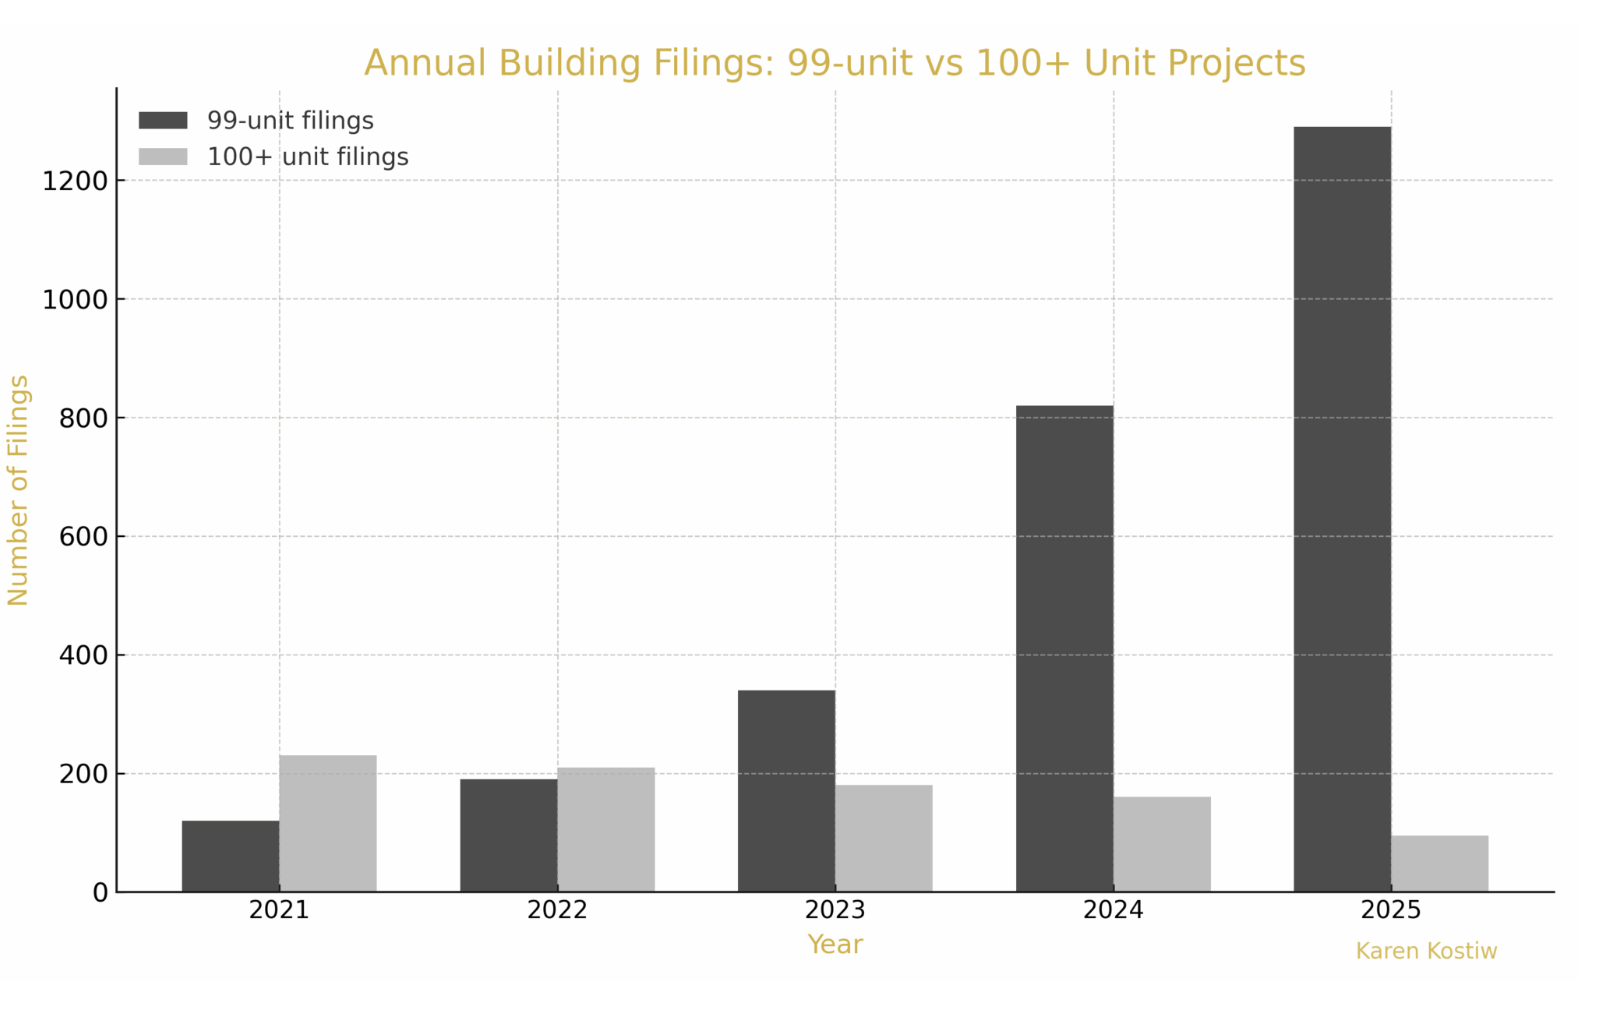
\includegraphics[width=\linewidth]{images/kostiw_99_unit_filings.png}
        \end{column}
    \end{columns}
\end{frame}

\begin{frame}
    \frametitle{Fewer Units or a Different Project Design?}
    \begin{itemize}[itemsep=0.5em]
        \item A 110-unit project cut to 99 loses 11 apartments
        \item The same project split into two buildings of 55 loses none
        \item A 210-unit project built as 99 + 99 loses 12
    \end{itemize}
    \vspace{0.5em}
    The housing cost of the threshold depends on which response developers choose.
\end{frame}

\begin{frame}
    \frametitle{This Paper}
    \begin{itemize}[itemsep=0.5em]
        \item Link new-building filings into parent projects, before and after 485-x
        \item Recent projects bunch at 99 units and at 99 + 99
        \item The share of projects split into several buildings rises
        \item A model of project size and splitting implies about \MainUnitsLost{} fewer proposed units among recent projects
    \end{itemize}
\end{frame}
